\documentclass{article}

%%%%%%%%%%%%%%%%%%%%%%%%%%%%%%%%%%%%%%%%%%%%%%%%%%%%%%%%%%%%%%%%%
%package

%geometry
\usepackage[a4paper]{geometry}%调整页面边距
\geometry{left=3cm,right=3cm,top=3cm,bottom=3cm}
\linespread{1.5}
\usepackage{fancyhdr}%梦幻页眉

%fonts
\usepackage{fontspec}%字体库
\defaultfontfeatures{Mapping=tex-text}
\usepackage{xunicode,xltxtra}
\usepackage[BoldFont,SlantFont,CJKnumber,CJKchecksingle]{xeCJK}  % \CJKnumber{12345}: 一万二千三百四十五
\usepackage{CJKfntef}
\usepackage{bm} %公式中的粗体字符\boldsymbol
\usepackage{pifont}

%color
\usepackage{color,xcolor}
\definecolor{GREEN}{RGB}{25,180,68}
\definecolor{YELLOW}{RGB}{255,255,224}
\definecolor{BLUE}{RGB}{9,148,234}
\definecolor{RED}{RGB}{139,0,0}
\definecolor{DRED}{RGB}{128,0,0}
\definecolor{GREY}{RGB}{128,128,128}
\usepackage[pagecolor={YELLOW}]{pagecolor}%设置页面底色
%http://www.toolskk.com/color.php

%math
\usepackage{amsmath,amsfonts,amssymb}

%graphics
\usepackage[americaninductors,europeanresistors]{circuitikz}
\usepackage{tikz}%可以绘制各种坐标图,方格图
\usetikzlibrary{positioning,arrows,shadows,shapes,calc,mindmap,trees,backgrounds}  % placements=positioning
\usepackage{graphicx}%\includegraphics插图命令
\usepackage{subfigure}  %%图形或表格并排排列

% table
\usepackage{colortbl,dcolumn}  %% 彩色表格
\usepackage{multirow}
\usepackage{multicol}
\usepackage{booktabs}

% code
\usepackage{fancyvrb}%漂亮的代码包
\usepackage{listings}%加入代码

% ref
\usepackage{hyperref}%扩展参考文献,目录功能和加入超链接。

% title
\usepackage{titlesec}%花哨的章节标题

\usepackage{etoolbox}
\makeatletter
\patchcmd{\ttlh@hang}{\parindent\z@}{\parindent\z@\leavevmode}{}{}
\patchcmd{\ttlh@hang}{\noindent}{}{}{}
\makeatother%titlesec旧版本无编号问题


\titleformat
{\section} % command
[display] % shape
{\bfseries\Large} % format
{第\ \thesection 章\ } % label
{0.3ex} % sep
{
    \rule{\textwidth}{1pt}
    \vspace{1ex}
    \centering
} % before-code
[
\vspace{-2ex}%
\rule{\textwidth}{1pt}
] % after-code


%tightly-packed lists
\usepackage{mdwlist}
\usepackage{verbatim}%comment命令的注释包
\usepackage{styles/zhfontcfg}%中文包
\usepackage{styles/visionouclistings}
\usepackage{styles/visionouccfg}

% head/foot
\setlength{\headheight}{15pt}

\fancyhf{}



%%%%%%%%%%%%%%%%%%%%%%%%%%%%%%%%%%%%%%%%%%%%%%%%%%%%%%%%%%%%%%%%%%%%%%

%settings
\setCJKmainfont{Adobe Kaiti Std} %设置为楷体
\setCJKmonofont{Adobe Fangsong Std}%仿宋
%页眉页脚


\makeatletter
\def\headrule{{\if@fancyplain\let\headrulewidth\plainheadrulewidth\fi%
\hrule\@height 2.5pt \@width\headwidth\vskip1pt%上面线为2.5pt粗  
\hrule\@height 0.5pt\@width\headwidth  %下面0.5pt粗            
\vskip-2\headrulewidth\vskip-1pt}      %两条线的距离        
\vspace{6mm}}     %双线与下面正文之间的垂直间距              
\makeatother         
 

% graphics
\graphicspath{{figures/}}
\tikzset{
    % Define standard arrow tip
    >=stealth',
    % Define style for boxes
    punkt/.style={
           rectangle,
           rounded corners,
           draw=black, very thick,
           text width=6.5em,
           minimum height=2em,
           text centered},
    % Define arrow style
    pil/.style={
           ->,
           thick,
           shorten <=2pt,
           shorten >=2pt,},
    % Define style for FlyZhyBall
    FlyZhyBall/.style={
      circle,
      minimum size=6mm,
      inner sep=0.5pt,
      ball color=red!50!blue,
      text=white,},
    % Define style for FlyZhyRectangle
    FlyZhyRectangle/.style={
      rectangle,
      rounded corners,
      minimum size=6mm,
      ball color=red!50!blue,
      text=white,},
    % Define style for zhyfly
    zhyfly/.style={
      rectangle,
      rounded corners,
      minimum size=6mm,
      ball color=red!25!blue,
      text=white,},
    % Define style for new rectangle
    nrectangle/.style={
      rectangle,
      draw=#1!50,
      fill=#1!20,
      minimum size=5mm,
      inner sep=0.1pt,}
}

% code
\lstnewenvironment{VHDLcode}[1][]{%
  \lstset{
    basicstyle=\footnotesize\ttfamily\color{black},%
    columns=flexible,%
    framexleftmargin=.7mm,frame=shadowbox,%
    rulesepcolor=\color{blue},%
%    frame=single,%
    backgroundcolor=\color{yellow!20},%
    xleftmargin=1.2\fboxsep,%
    xrightmargin=.7\fboxsep,%
    numberstyle=\tiny\color{blue},%
    numberblanklines=false,numbersep=7pt,%
    language=VHDL%
    }\lstset{#1}}{}
\lstnewenvironment{VHDLmiddle}[1][]{%
  \lstset{
    basicstyle=\scriptsize\ttfamily\color{black},%
    columns=flexible,%
    framexleftmargin=.7mm,frame=shadowbox,%
    rulesepcolor=\color{blue},%
%    frame=single,%
    backgroundcolor=\color{yellow!20},%
    xleftmargin=1.2\fboxsep,%
    xrightmargin=.7\fboxsep,%
    numbers=left,numberstyle=\tiny\color{blue},%
    numberblanklines=false,numbersep=7pt,%
    language=VHDL%
    }\lstset{#1}}{}
\lstnewenvironment{VHDLsmall}[1][]{%
  \lstset{
    basicstyle=\tiny\ttfamily\color{black},%
    columns=flexible,%
    framexleftmargin=.7mm,frame=shadowbox,%
    rulesepcolor=\color{blue},%
%    frame=single,%
    backgroundcolor=\color{yellow!20},%
    xleftmargin=1.2\fboxsep,%
    xrightmargin=.7\fboxsep,%
    numbers=left,numberstyle=\tiny\color{blue},%
    numberblanklines=false,numbersep=7pt,%
    language=VHDL%
    }\lstset{#1}}{}
% pdf
\hypersetup{pdfauthor={Haiyong Zheng},%
            pdftitle={Title},%
            CJKbookmarks=true,%
            bookmarksnumbered=true,%
            bookmarksopen=false,%
            plainpages=false,%
            colorlinks=true,%
            citecolor=green,%
            filecolor=magenta,%
            linkcolor=DRED,%red(default)
            urlcolor=cyan}
\newcommand\titlebar{%
\tikz[baseline,trim left=3.1cm,trim right=3cm] {
    \fill [cyan!25] (2.5cm,-1ex) rectangle (\textwidth+3.1cm,2.5ex);
    \node [
        fill=cyan!60!white,
        anchor= base east,
        rounded rectangle,
        minimum height=3.5ex] at (3cm,0) {
        \textbf{\thesection.}
    };
}%
}

%code
\definecolor{mygreen}{rgb}{0,0.6,0}
\definecolor{mygray}{rgb}{0.5,0.5,0.5}
\definecolor{mymauve}{rgb}{0.58,0,0.82}
\lstset{
 backgroundcolor=\color{white}, 
 basicstyle = \footnotesize,       
 breakatwhitespace = false,        
 breaklines = true,                 
 captionpos = b,                    
 commentstyle = \color{mygreen}\bfseries,
 extendedchars = false,             
 frame =shadowbox, 
 framerule=0.5pt,
 keepspaces=true,
 keywordstyle=\color{blue}\bfseries, % keyword style
 language = C++,                     % the language of code
 otherkeywords={string}, 
 numbers=left, 
 numbersep=5pt,
 numberstyle=\tiny\color{mygray},
 rulecolor=\color{black},         
 showspaces=false,  
 showstringspaces=false, 
 showtabs=false,    
 stepnumber=1,         
 stringstyle=\color{mymauve},        % string literal style
 tabsize=2,          
 title=\lstname                      
}


%设置标题页面

\newcommand*{\titleGM}{\begingroup % 新命令:添加标题页
\hbox{ % 水平盒子
\hspace*{0.2\textwidth} % 左边空白
\rule{1pt}{\textheight\color{GREY}} % 竖线
\hspace*{0.05\textwidth} % 竖线和文本距离
\parbox[b]{0.75\textwidth}{ % 文本最大右边距

{\noindent\Huge\bfseries \LaTeX \\[0.5\baselineskip] - Getting Started}\\[2\baselineskip] % 题目
{\large \textit{一份\LaTeX 入门手册}}\\[4\baselineskip] % 标签或描述
{\Large \textsc{丁昊}}\\ % 作者

\vspace{0.5\textheight} % 题目区域和作者间距
{\noindent August 2016 }\\[\baselineskip] % Publisher and logo
}}
\endgroup}


                      
\chead{\color{GREY}\LaTeX-GETTING STARTED}%页眉
\cfoot{\color{GREY}August 2016}%页脚 中
\lfoot{\color{GREY}DingHao}%页脚 左
\rfoot{\color{GREY}$\cdot$\ Page \thepage\ }%页脚 右
\renewcommand{\headrulewidth}{0.4pt}
\renewcommand{\footrulewidth}{0.4pt}

\usepackage{styles/lshort}

%%%%%%%%%%%%%%%%%%%%%%%%%%%%%%%%%%%%%%%%%%%%%%%%%%%%%%%%%%%%%%%%%
\begin{document}

\titleGM\thispagestyle{empty}

\pagenumbering{roman}

\setcounter{page}{0}
\newpage

\begin{abstract}
这篇文档作者写的虽然是我的名字,事实上却是因为我很难把那么多名字统统写进来。首先,本文档后半部分内容主要来源于孙雪,戴嘉伦两位师兄师姐和郑海永老师的《\LaTeX 简短使用手册》。版式的设置部分参照了常琳师姐的文档模板,并采取了崔金娜、谭琳和王超的很多建议。写这篇文档的过程对我也是个挑战,郑老师帮我解决了一系列编写中遇到的问题。且本文的绝大部分实际内容来自于官方编写的《一份不太简短的\LaTeXe 介绍》(后文简称为《介绍》),所以说我实际上是做了大量整理工作而非原创性工作。\par
但是到目前为止,上面提到的这些及网上的文档要不太长,要不难以满足翻遍电脑找不到\LaTeX 可执行文件在哪的初学级菜鸟的需求,我尽我最大的努力给予一些我在那个阶段最想要知道的一些信息,尽量的总结至一天可以学会的量,而不再需要你们将一整天又一整天的时间耗费在百度和谷歌上。\par
最后,我个人的水平着实有限,希望这份文档可以被不断的修改和更新,并以更好的样子服务更多的师弟师妹。
\end{abstract}

\newpage

\tableofcontents 
\newpage

\pagestyle{fancy}

\pagenumbering{arabic}
\newpage
                      

%%%%%%%%%%%%%%%%%%%%%%%%%%%%%%%%%%%%%%%%%%%%%%%%%%%%%%%%%%%%%%%%

\section{\LaTeX 简介}

\subsection{发展}

\TeX 最初是Donald E. Knuth编写的,它可以完美的适应不同电脑,并能够满足用户对排版要求的几乎全部需求。但上世纪的\TeX 版本对用户的友好度比较低,语句繁琐且晦涩难通。直到Leslie Lamport对其进行了整理,制作出新的宏集,也就是我们如今使用的这个方便易学的\LaTeX 。

\subsection{我们为什么学习\LaTeX ?}

习惯于Windows界面的我们,为什么要踏上Linux的不归路?最适应Word的我们,为什么非要使用\LaTeX ?除了导师或未来公司有相应要求,我个人认为主要有以下几点:

\begin{itemize}
\item 无论是Windows系统还是Office软件,都是有能力与计算机自由交谈的程序员们,为了让现今社会绝大部分的普通人,都能便捷的使用计算机这一现代科技,而在人与电脑之间辛苦构建起的宏大桥梁。这些界面华丽的系统和软件,一切以便利为主,人们无需多做思考就能得到希望得到的讯息。可是就如同我们要学习C、Matlab等各种语言一样,我们希望自己有能力与计算机面对面沟通。已经制作好的软件功能一定是有限的,可是放在一个开源的世界,我们想到什么,就可以做到什么。有了“渔”的本领,想要得到“鱼”,岂不是手到擒来。

\item 在信息这个如此大范畴的领域当中,我们难以望其项背的大神们,每一个都拥有畅游开源世界的能力。如果软件出现bug,闭源的Windows只允许你提交反馈,反馈量的巨大使得问题长时间无人修复,相同的事情出现在Linux,我们除了给创始人发送邮件和去贴吧吐槽之外,还可以自己修改代码,或改进功能。自己成为系统更新者之一,是不是听起来就很赞?

\item 说了这么多,接下来讲讲\LaTeX 相较Word的优势。首先是文档自动排版功能,用户只能使用结构化的方式写作,这使得输出的PDF结构非常的清晰。自定义宏包和公式的功能使得\LaTeX 无限的强大,有能力输出任何你想得到的排版方式。数学公式自动编号与代码的便利编写对我们专业的好处更不必说。网上看到一个很有意思的总结贴在这里:不会用Word得到很丑的文档,不会用\LaTeX 没有文档;会用Word得到文档,会用\LaTeX 得到漂亮的文档;用的好,Word和\LaTeX 都可以得到牛逼的文档。
\end{itemize}
\newpage
%%%%%%%%%%%%%%%%%%%%%%%%%%%%%%%%%%%%%%%%%%%%%%%%%%%%%%%%%%%%%%%%
\section{快速上手}

\subsection{创建与使用}

相信看到这里,你已经装好\LaTeX 并信心满满的准备使用了,如果没有,请去阅读LaTeX-install.pdf。

首先我们来创建一个文档,位置随你,我的选择是在~/TeXLive文件夹下集中管理我的所有\LaTeX 文档。这里有一个小建议,因为每份\LaTeX 文档生成过程中,都会同时产出几个附加文档,所以你写的每个文档最好放在不同的文件夹下。下面所有的操作都推荐像我一样使用终端来进行控制。

1.来到该目录下:
\begin{verbatim}
       cd ~/TeXLive/
\end{verbatim}


2.创建test文件夹
\begin{verbatim}
       mkdir test
\end{verbatim}


3.创建test.tex文件
\begin{verbatim}
       touch test.tex      [LaTeX文档都要写成这个后缀]
\end{verbatim}


4.编辑test.tex
\begin{verbatim}
       gedit test.tex      [郑老师强力推荐使用vim而不是gedit]
\end{verbatim}


5.在打开的文件中输入:
\begin{verbatim}
       \documentclass{article}
       \begin{document}
       Hello!World!
       \end{document}
\end{verbatim}


6.编译该文件【请重复这个步骤2到3次,因为\LaTeX 往往需要2到3次编译才能正确呈现目录】
\begin{verbatim}
       xelatex test.tex    [使用这个命令要在.tex文件所在的目录下哦~]
\end{verbatim}


7.成功导出PDF文档
\begin{verbatim}
       Hello!World!
\end{verbatim}


\ding{80}记住以上步骤,以后的编译过程都是这样去做的。

\subsection{基本语句解析}
\LaTeX 存在固定的格式,总体分为:文档定义、宏包说明、格式设置、正文这四个部分。由于\LaTeX 本身自带默认的宏包和设置,这两个部分不是必须的。

\subsubsection{文档定义:}
\begin{verbatim}
  \documentclass[options]{class}  
  [这是一个标准的语句描述,方括号允许整个去掉,大括号不行。]
  [有些情况大括号内容存在默认设置且你想要使用默认,可以写一个{}来略过该设置]
\end{verbatim}
\begin{itemize}
\item options:用来调整字体大小,单面双面,纸张大小,公式对齐方式等等。
\item class:标注文档类型,不同文档可以使用的宏包和语句都有些许区别。常用的有article(短报告、程序文档、本篇给你们的小教程),report(毕业论文等长报告),book(书),slides(幻灯片)。
\item Example: $\backslash$documentclass[11pt,twoside,a4paper]\{article\}表示该文档排版为11磅字体的article格式,并得到A4纸上双面打印的效果。
\end{itemize}
以上已经够用,更详细说明见《介绍》Page8-表1.1,表1.2。

\subsubsection{宏包说明与格式设置:}
\begin{verbatim}
  \usepackage[options]{package}
\end{verbatim}\\

每一份文档都可以使用无数量限制的宏包,通常情况下,\LaTeX 自带的宏包足够使用,若希望自己添加一个宏包,可以编写或下载一个name.sty文件,并放在与.tex文件相同的路径下,这时在宏包说明部分添加$\backslash$usepackage\{name\}便可调用。如LaTeX-install中添加的zhfontcfg.sty就是一个自己配置的中文包。\par
设置部分多是使用前面已添加的宏包进行一些排版上的调整,比如添加了color这个包,你就可以使用$\backslash$definecolor\{GREEN\}\{RGB\}\{25,180,68\}指令来设置一个\LaTeX 不自带的颜色。事实上\LaTeX 可以做到完全自由,你可以自己去编写个性的命令或环境以应用于你的文档,但这已不属于初级的入门教程,感兴趣请查阅《介绍》Page83-第六章内容。\par
当然,你完全可以复制已写好的\LaTeX 模板来编写自己的文档,这样做可以省略整个宏包的配置与设置过程。\par
下面对常用宏包作一下简短的介绍:
\begin{itemize}

\item geometry:调整页面边距、行距等
\item titlesec:更改各级标题样式(该宏包在2016版Texlive自带的版本存在使文档丢失序号的问题,需要添加一段代码或自行下载新版进行更新后使用)
\item fancyhdr:更改更多页眉页脚设置
\item fontspec:字体库
\item color,xcolor:添加更多颜色
\item pagecolor:设置页面底色
\item amsmath,amsfonts,amssymb:一些数学公式包,可设置公式格式,编号等
\item graphicx:插入图像
\item listings:插入代码
\item hyperref:扩展参考文献,目录功能和加入超链接
\item verbatim:命令注释包,即调用后可即时输出特殊字符等
\item zhfontcfg:中文包

\end{itemize}\par
以上只是我认为较为重要的,欢迎补充。想要学习更多的宏包设置知识,不要去看类似宏包大全的网页,但需要你对照某个文档的宏包部分,针对想弄懂的宏包去search,并尽量自己一点一点的试验不同设置下的输出区别,本篇文档的该部分作了一些不太完整的说明,希望能够帮到你。

\subsubsection{正文}
\LaTeX 的正文必须写在$\backslash$begin\{document\}和$\backslash$end\{document\}之间。一般来说,一篇article的组成无外乎标题、作者、日期、目录、摘要、分章节说明等部分。下面逐一列举了语句写法。\par
\begin{itemize}
\item 标题:\qquad \qquad $\backslash$title\{标题名称\}
\item 作者:\qquad \qquad $\backslash$author\{作者\}
\item 日期:\qquad \qquad $\backslash$date\{2016年7月\}
\item 添加标题:\qquad $\backslash$maketitle
\item 添加目录:\qquad $\backslash$tableofcontents
\item 摘要:\qquad \qquad $\backslash$begin\{abstract\} 摘要内容 $\backslash$end\{abstract\}
\item 章节:\qquad \qquad $\backslash$section\{章节\} $\backslash$subsection\{次级章节\} $\backslash$subsubsection\{三级章节\}
\item 段落:\qquad \qquad $\backslash$paragraph\{段落\} $\backslash$subparagraph\{次级段落\}
\item 分节:\qquad \qquad $\backslash$part\{分块而不影响章节编号\}
\item 大章节:\qquad \quad $\backslash$chapter\{仅使用于report和book文档\}

\end{itemize}
请不要着急,以上只是对正文部分最主要成分的列举,详细语句规则往下看。
\newpage
%%%%%%%%%%%%%%%%%%%%%%%%%%%%%%%%%%%%%%%%%%%%%%%%%%%%%%%%%%%%%%%%
\section{\LaTeX 书写规则与常用命令}

\subsection{书写规则}
\subsubsection{文章分区与断行}
\begin{enumerate}%空格
\item 多个连续空格被视为一个空格,一个空白行(两个回车)表示另起一段,多个连续空行被视为一个空行:

\begin{example}
It does not matter whether you enter one
 or several       spaces after a word.


An empty line starts a new paragraph.
\end{example}

\item \LaTeX 的几个换行命令:[\textsl{这里这个展示环境没有做好,事实上前两个另起一段的命令开头是会产生两个缩进的}]%换行

\begin{example}
输入\par 或者两个回车

可以另起一段;输入\\或者
\newline 可以强制断行(不缩进);
输入\\*表示强制断行且禁止分页;
$\backslash$newpage 表示另起一页
\end{example}

\item 百分号后的本句内容被视为注释,不在PDF显示,长注释可使用comment环境:

\begin{example}
%短注释
\begin{comment}
长注释
\end{comment}  
\end{example}
\end{enumerate}

\subsubsection{特殊字符}

\begin{enumerate}
\item \LaTeX 中有许多特殊字符不能够直接输出,下面几个常用的保留字符可以通过加反斜杠输出,其他特殊字符可以通过特殊命令得到%特殊字符

\begin{example}
\# \$ \% \^ \& \_ \{ \} $\backslash$
\end{example}

\item 内置字符串

\begin{example}
\today 

\TeX

\LaTeX

\LaTeXe
\end{example}

\item 横杠

\begin{example}
daughter-in-law 连字号

pages 13--67 短破折号

yes---or no? 长破折号

$-1$ 减号
\end{example}

\item 波浪号

\begin{example}
http://rich.edu/$\sim$demo
\end{example}

\item 度的符号

\begin{example}
$-30\,^{\circ}\mathrm{C}$
\end{example}

\item 欧元符号

\begin{example}
\texteuro
\end{example}

\item 省略号

\begin{example}
\ldots
\end{example}

\item 禁止断词

\begin{example}
shelf\mbox{}ful  这个单词不会被断开
加连字符到下一行
\end{example}

\item 注音符号和特殊字符

\begin{example}
H\^otel, na\"\i ve\\
sm\o rrebr\o d, !'Se\ norita!\\
Sch\"onbrunner Schlo\ss{}
Stra\ss e
\end{example}

\end{enumerate}

%%%%%%%%%%%%%%%%%%%%%%%%%%%%%%%%%%%%%%%%%%%%%
\subsection{格式}

\begin{enumerate}
\item 命令后加空格需要一对大括号
\begin{example}
\TeX{} I 
\end{example}

\item 设置斜体
\begin{example}
\textsl{斜体} 
\end{example}

\item 脚注
\begin{example}
Footnotes\footnote{This is a footnote.}
 are often used by people using \LaTeX.
\end{example}

\item 强调
\begin{example}
\underline{下划线}

\emph{印刷品用斜体字体排印要强调的单词}
\end{example}
\end{enumerate}

\subsection{环境}
\subsubsection{排版}

\begin{enumerate}
\item 编号:itemize、enumerate、description用法
\begin{example}
\begin{enumerate} %条目
\item You can mix the list environments 
 to your taste:
\begin{itemize}
\item But it might start to look silly.
\item[-] With a dash.
\end{itemize}
\item Therefore remember:
\begin{description}
\item[Stupid] things will not become 
smart because they are in a list.
\item[Smart] things, though, can be 
presented beautifully in a list.
\end{description}
\end{enumerate}
\end{example}

\item 对齐
\begin{example}
\begin{flushleft}
左对齐
\end{flushleft}
\begin{flushright}
右对齐
\end{flushright}
\begin{center}
居中对齐
\end{center}
\end{example}

\subsubsection{插入}
\item 引用、语录和韵文
\begin{example}
一个例子:
\begin{quote}
一定要认真阅读例子,因为在贯穿全篇的各种
例子里包含了很多的信息。
\end{quote}
例子结束
\end{example}

\item 表格
\begin{itemize}
	\item 代码
\begin{verbatim}
\begin{table}[!htp] %插表
\label{tab:1}
\centering
\begin{tabular}{|c|c|c|c|}
\hline
0.5&0&0&0\\
\hline
0&1&0&0\\
\hline
0&0.25&0.75&0\\
\hline
0&0&0&1\\
\hline
\end{tabular}  
\caption{一个表格}
\end{table}
通过表\ref{tab:1},我们可以得出\ldots
\end{verbatim}
	\item 输出\\
\begin{table}[!htp] %插表
\label{tab:1}
\centering
\begin{tabular}{|c|c|c|c|}
\hline
0.5&0&0&0\\
\hline
0&1&0&0\\
\hline
0&0.25&0.75&0\\
\hline
0&0&0&1\\
\hline
\end{tabular}  
\caption{一个表格}
\end{table}
通过表\ref{tab:1},我们可以得出\ldots
\end{itemize}

\item 插图
\begin{itemize}
	\item 代码
\begin{verbatim}
\begin{figure}[!htb] %插图
\centering
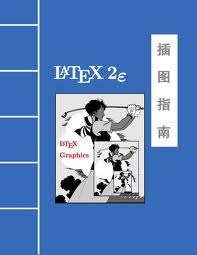
\includegraphics[width=0.5\textwidth]{latex_figure.jpeg}
\caption{\LaTeX{}插图指南}
\label{fig:1}
\end{figure}
通过图\ref{fig:1},我们可以得出\ldots
\end{verbatim}
	\item 输出\\
\begin{figure}[!htb] %插图
\centering
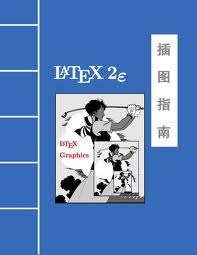
\includegraphics[width=0.5\textwidth]{latex_figure.jpeg}
\caption{\LaTeX{}插图指南}
\label{fig:1}
\end{figure}
通过图\ref{fig:1},我们可以得出\ldots
\end{itemize}

\end{enumerate}
\newpage
%%%%%%%%%%%%%%%%%%%%%%%%%%%%%%%%%%%%%%%%%%%%%%



\section{数学公式}

\subsection{行间式样}
\begin{itemize}
\item 和的平方
\begin{example}
$c^{2}=a^{2}+b^{2}$
\end{example}
\item 心型
\begin{example}
\begin{math}\heartsuit\end{math}
\end{example}
\item 极限
\begin{example}
$\lim_{n \to \infty}\sum_{k=1}^n \frac{1}{k^2} = \frac{\pi^2}{6}$
\end{example}
\end{itemize}

\subsection{显示式样}
\begin{itemize}
\item 求$a$与$b$的和
\begin{example}
\begin{displaymath}
a+b=c
\end{displaymath}
\end{example}
\item 和的平方
\begin{example}
\[c^{2}=a^{2}+b^{2}\]
\end{example}
\item 极限
\begin{example}
\begin{displaymath}
\lim_{n \to \infty}
\sum_{k=1}^n \frac{1}{k^2}
= \frac{\pi^2}{6}
\end{displaymath}
\end{example}
\end{itemize}

\subsection{公式编号}
\begin{example}
\begin{equation} \label{eq:eps}
\epsilon > 0
\end{equation}
\end{example}
从公式(\ref{eq:eps}), 我们得出\ldots

\subsection{数学模式的群组}
\begin{example}
\begin{equation}
a^x+y \neq a^{x+y}
\end{equation}
\end{example}

\subsection{数学公式的基本元素}

\begin{enumerate}

\item 希腊字母

\begin{example}
$\alpha, \beta, \gamma, \Gamma, \Delta, 
\lambda, \xi, \pi, \mu, \Phi, \Omega$
\end{example}
\newpage
\item 指数和下标
\begin{example}
$a_{1}$, $e^{x^2}\neq {e^x}^2$
\end{example}
\item 平方根
\begin{example}
$\sqrt{x}$, $\sqrt[3]{2}$ 
\end{example}
\item 水平线
\begin{example}
$\overline{m+n}$, $\underline{m+n}$
\end{example}
\item 水平括号 
\begin{example}
$\underbrace{a+b+\cdots+z}_{26}$
\end{example}
\item 导数
\begin{example}
$y=x^{2}\qquad y’=2x\qquad y’’=2$
\end{example}
\item 乘号
\begin{example}
$x_{1}\cdot x_{2}$
\end{example}
\item log等类的函数名通常用直立字体
\begin{example}
\begin{flushleft}$\arccos, \cos, \csc, 
\exp, \ker, \limsup,\arcsin, \cosh,$\\$
 \deg, \gcd, \lg, \ln, \arctan \cot 
\det, \hom, \lim, \log,\arg,$\\$ \coth, 
\dim, \inf, \liminf, \max, \sinh, \sup, 
\tan \tanh, $\\$\min, \Pr,\sec, \sin$ 
如极限:$\lim_{x \rightarrow 
0}\frac{\sin x}{x}=1$
\end{flushleft}
\end{example}
\item 取模函数
\begin{example}
$a\bmod b$, $x\equiv a \pmod{b}$
\end{example}
\item 分式
\begin{example}
$1\frac{1}{2}$, $\frac{x^2}{k+1}$, $1/2$
\end{example}
\item 二项式系数
\begin{example}
$\binom{n}{k},\mathrm{C}_n^k$
\end{example}
\item 符号堆积
\begin{example}
$\stackrel{!}{=}$
\end{example}
\item 积分号,累加,累乘
\begin{example}
$\int_{0}^{\frac{\pi}{2}} \qquad 
\sum_{i=1}^{n} \qquad \prod_\epsilon$
\end{example}
\item 括号

\begin{itemize}
\item 自动调整括号尺寸 
\begin{example}
\begin{displaymath}
1 + \left( \frac{1}{ 1-x^{2} }
\right) ^3
\end{displaymath}
\end{example}
\item 指定括号尺寸
\begin{example}
$\big(\Big(\bigg(\Bigg($\quad$\big\}\Big\}\bigg\}\Bigg\}$\quad
$\big\|\Big\|\bigg\|\Bigg\|$
\end{example}
\end{itemize}

\item 竖直点列,对角线点列
\begin{example}
$\vdots\quad \ddots$
\end{example}
\end{enumerate}

\subsection{垂直取齐}

\begin{enumerate}
\item 括号中垂直取齐
\begin{example}
\begin{displaymath}
\mathbf{X} =
\left( \begin{array}{ccc}
x_{11} & x_{12} & \ldots \\
x_{21} & x_{22} & \ldots \\
\vdots & \vdots & \ddots
\end{array} \right)
\end{displaymath}
\end{example}

\begin{example}
\begin{displaymath}
y = \left\{ \begin{array}{ll}
a & \textrm{if $d>c$}\\
b+x & \textrm{in the morning}\\
l & \textrm{all day long}
\end{array} \right.
\end{displaymath}
\end{example}

\begin{example}
\begin{displaymath}
\left(\begin{array}{c|c}
1 & 2 \\
\hline
3 & 4
\end{array}\right)
\end{displaymath}
\end{example}

\item 等号取齐:
\begin{example}
\begin{eqnarray}
f(x) & = & \cos x
\\
f’(x) & = & -\sin x
\\
\int_{0}^{x} f(y)dy &
= & \sin x
\end{eqnarray}
\end{example}

\item 长等式指定在哪断和如何缩进:
\begin{example}
{\setlength\arraycolsep{2pt}
\begin{eqnarray}
\sin x & = & x -\frac{x^{3}}{3!}
+\frac{x^{5}}{5!}-{}
\nonumber\\
&& {}-\frac{x^{7}}{7!}+{}\cdots
\end{eqnarray}}
\end{example}

\begin{example}
\begin{eqnarray}
\lefteqn{ \cos x = 1
-\frac{x^{2}}{2!} +{} }
\nonumber\\
& & {}+\frac{x^{4}}{4!}
-\frac{x^{6}}{6!}+{}\cdots
\end{eqnarray}
\end{example}
\end{enumerate}

\subsection{虚位}
\begin{example}

${}^{12}_{\phantom{1}6}\textrm{C} 
\qquad {}^{12}_{6}\textrm{C} $

$\Gamma_{ij}^{\phantom{ij}k} 
\qquad \Gamma_{ij}^{k} $ 
\end{example}

\subsection{定理、定律}

\begin{example}
\newtheorem{law}{Law} %定理
\begin{law}\label{law:t} 
This is my interesting theorem.
\end{law}
通过定理\ref{law:t},我们得出\ldots
\begin{proof}
\[E=mc^2\]
\end{proof}
\end{example}
\subsection{粗体符号}

\begin{example}
\begin{displaymath}
\mu, M \qquad
\boldsymbol{\mu}, \boldsymbol{M}
\end{displaymath}
\end{example}
\newpage
%%%%%%%%%%%%%%%%%%%%%%%%%%%%%%%%%%%%%%%%%%%5

\section{代码高亮}

\subsection{C++}
\begin{lstlisting}[caption={}]
#include "randomGenerator.h"
void normalNumGen(double mean, double sd,
                  int num, string filename){
	const int nrolls=num; // number of eperiments
	default_random_engine generator;
	normal_distribution<double> dnorm(mean, sd);
	ofstream outfile(filename,ios::out);
	for(int i=0; i < nrolls; ++i){
		double number = dnorm(generator);
		outfile << number << endl;
	}
}
\end{lstlisting}

\subsection{Matlab}

\lstinputlisting{matlab_code.m} %插入Matlab代码({}中为代码地址)

\subsection{python}

\begin{lstlisting}
for i = 1:3
\end{lstlisting}

\begin{python}
#!/usr/local/bin/python
print "Hello World"
os.system("""
VAR=even;
sed -i "s/$VAR/odd/" testfile;
for i in `cat testfile` ;
do echo $i; done;
echo "now the tr command is removing the vowels";
cat testfile |tr 'aeiou' ' '
""") 
\end{python}

\subsection{bash}

\begin{bash}
#!/bin/bash
if [ $# == 1 ]; then
    echo -ne "Deleting FILES including [$1] in the CURRENT directory ...\n\n"
    for i in $(tree -a -f -i | grep "$1")
    do
      echo -ne "Deleting $i\n"
      rm -f $i
    done
elif [ $# == 2 ]; then
    echo -ne "Deleting FILES including [$1] in [$2] directory ...\n"
    for i in $(tree -a -f -i $2 |grep "$1")
    do
      echo -ne "Deleting $i\n"
      rm -f $i
    done    
else
    echo -ne "Arguments Error.\n"
    echo -ne "Usage:\n"
    echo -ne "\t$0 STRING\n"
    echo -ne "\t$0 STRING DIRECTORY\n"
fi
cd ~/
\end{bash}

\subsection{plain}

\begin{plaintext}
user = zhenghaiyong
email = zhenghaiyong@gmail.com
\end{plaintext}

% references
\bibliographystyle{plain}

\bibliography{template} %参考文献




\end{document}
